\documentclass[fleqn]{jbook}
\usepackage{physpub}
% amsmath, graphicx は自動的に読み込まれるので
% \usepackage しないでください、してもかまわないけど。
\begin{document}

\begin{question}{問題8}{菅原・永村}

図1はヒトの眼の断面図である。眼に入射する光は、まず空気と角膜との境界面で屈折し、さらに水晶体の前面と後面で2度屈折し、網膜上に像を結ぶ。網膜上で光は電気信号におきかえられ、視覚情報として視神経を通して脳に伝えられる。

\begin{figure}[htbp]
\begin{center}
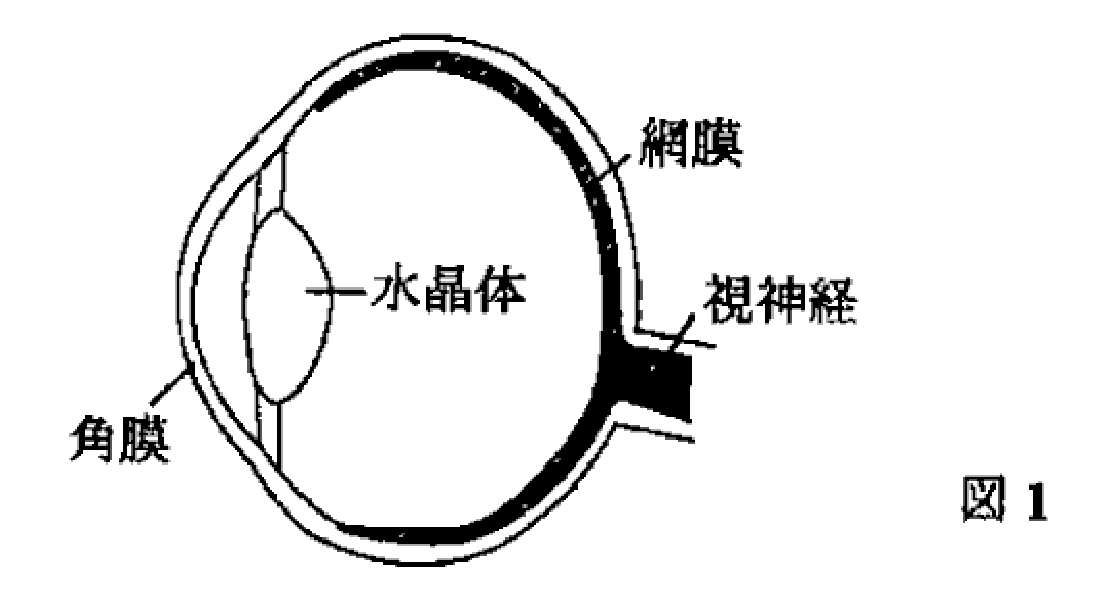
\includegraphics[width=70mm]{2003phy8-1.eps}
\end{center}
\end{figure}

まず光学機器として眼をとらえよう。ヒトの眼全体で起こる光の屈折の大部分は空気と角膜の境界面で生じている。水晶体における屈折を無視した時の、角膜による像形成(図2)を考える。物体OO'と角膜との距離を$p$、角膜と像の形成位置Iとの距離を$q$、空気中および角膜内の屈折率を$n_1$、$n_2$とする。角膜表面を球面の一部とみなし、その中心をC、半径を$r$とする。

\begin{figure}[htbp]
\begin{center}
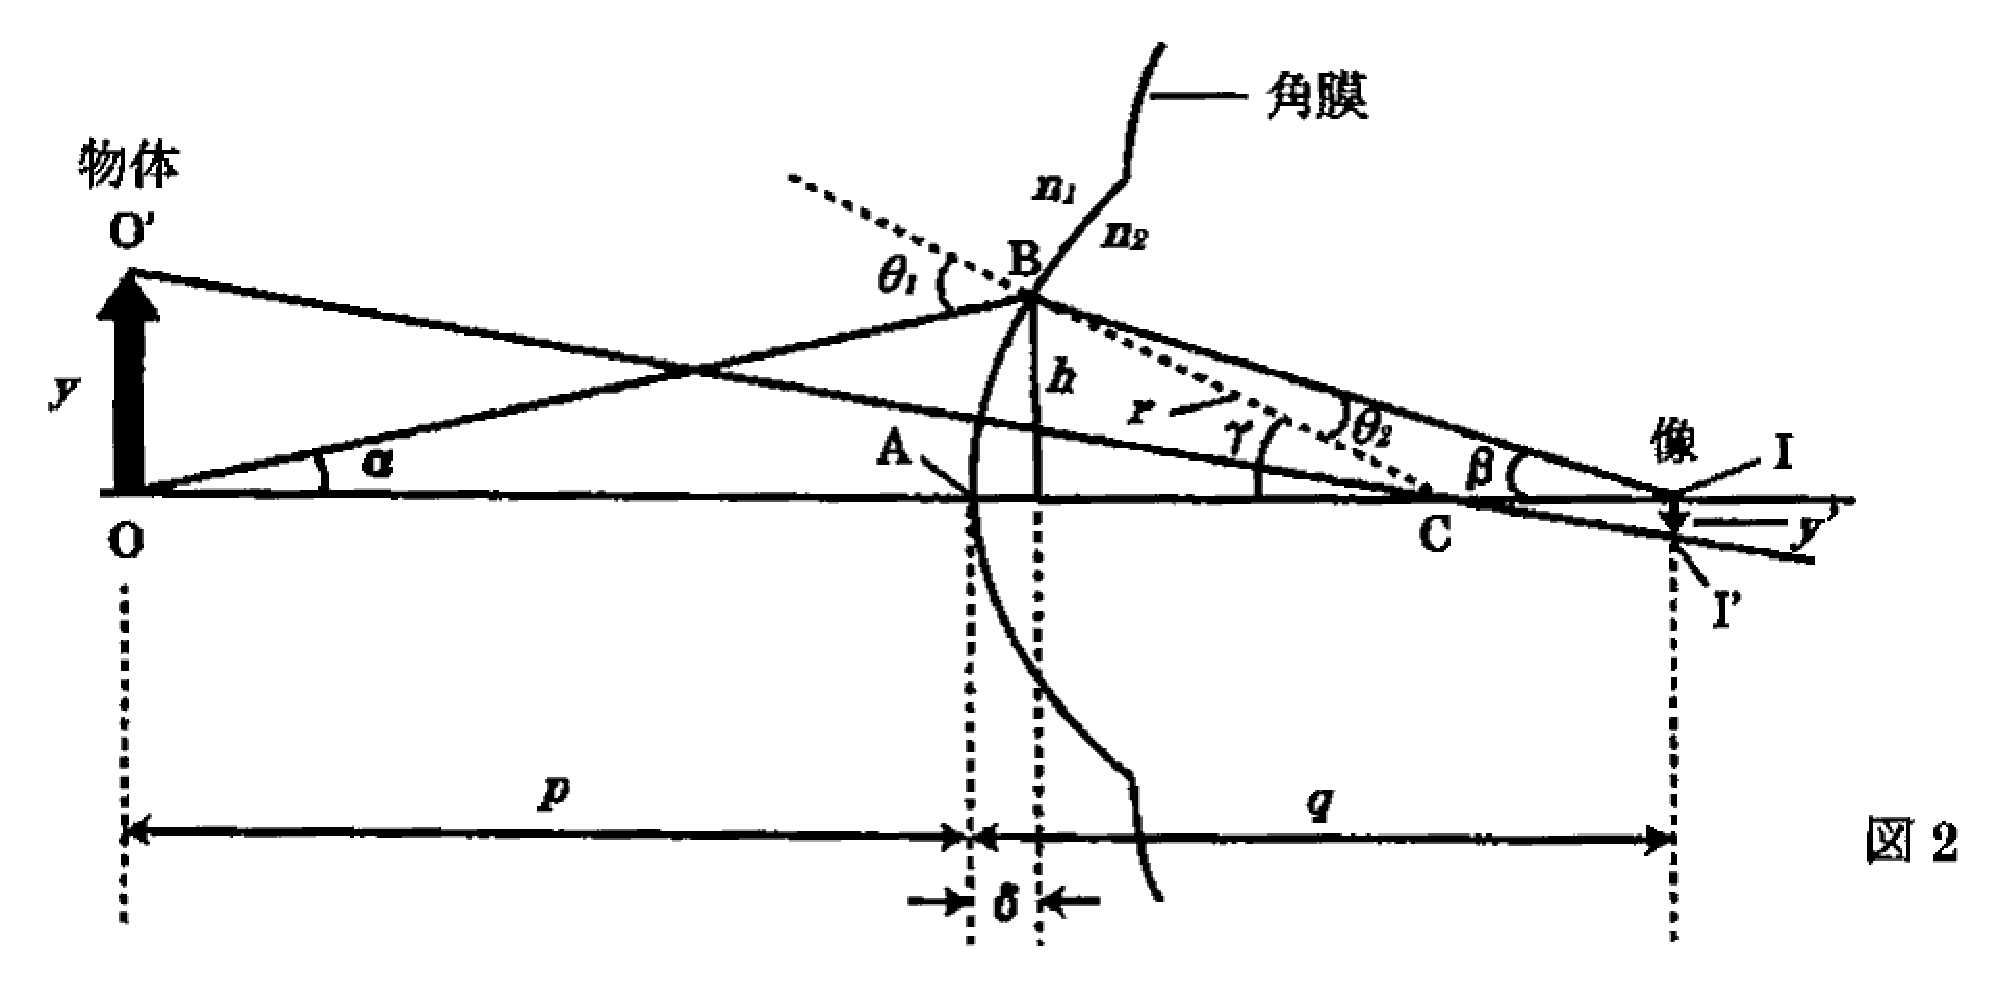
\includegraphics[width=140mm]{2003phy8-2.eps}
\end{center}
\end{figure}

\begin{enumerate}
\item 光線OBIに着目する。点Bと直線OIとの距離を$h$とし、図中の角$\alpha$(∠BOI)、$\beta$(∠BIO)、$\gamma$(∠BCO)を$h$、$p$、$q$、$r$で表せ。なお、図中の距離$\delta$は$p$、$q$、$r$に比べて無視できるものとし、$\alpha$、$\beta$、$\gamma \ll 1$ラジアンとする。
\item 光線OBIの入射角、屈折角を$\theta_1$、$\theta_2$とし、$\theta_1$、$\theta_2$、$n_1$、$n_2$間の関係式を示せ。ただし、$\theta_1$、$\theta_2 \ll 1$ラジアンとする。
\item 設問1、2より$n_1$、$n_2$、$p$、$q$、$r$間の関係式を求めよ。
\item 網膜における像の拡大率$m$($= y'/y$)を$n_1$、$n_2$、$p$、$q$で表せ。
\item $p=25$cm、$p= \infty$の時、$q$の値をそれぞれ有効数字2桁で求めよ。ただし、$n_1 = 1.00$、$n_2 = 1.34$、$r = 0.80$cmである。
\item 設問5で求めた$q$の値と角膜と網膜との間の実際の距離$2.5$cmを比べることにより、どのようなことが分かるか。水晶体の役割を含め説明せよ。
\end{enumerate}

次に網膜上の像が視神経を介し脳へと投射される過程を考察する。
\begin{enumerate}\setcounter{enumi}{6}
\item 各視神経は図3の点Aと点A'、点Bと点B'といった具合に、網膜上の特定の点と1次視覚野上の対応する点とを結ぶように配線される。このように各視神経が網膜上での相対的な位置を保ったままで1次視覚野に結合する結果、脳内において網膜上の像が再現される。カエルの視神経が、図3で示すような位置で切断されても再生する能力を持つことを利用し、視神経の正確な配線のパターンが遺伝的に決定されているのか、それとも学習によって獲得されるのかを検討する実験を考案せよ。
\item 実際には視神経の配線は、大部分、遺伝的に決定されていることがわかっている。したがって、各視神経と1次視覚野の特定の位置とを対応づける分子の存在が予想される。もし、このような分子(遺伝子にコードされていると仮定する)が視神経の数だけ必要であるとすると、遺伝子の数が断然不足することになる(視神経の数は100万のオーダーであるのに対し、ヒトの遺伝子の数は数万しかない)。この問題を回避するため生物がとっている戦略について考察せよ。

\begin{figure}[htbp]
\begin{center}
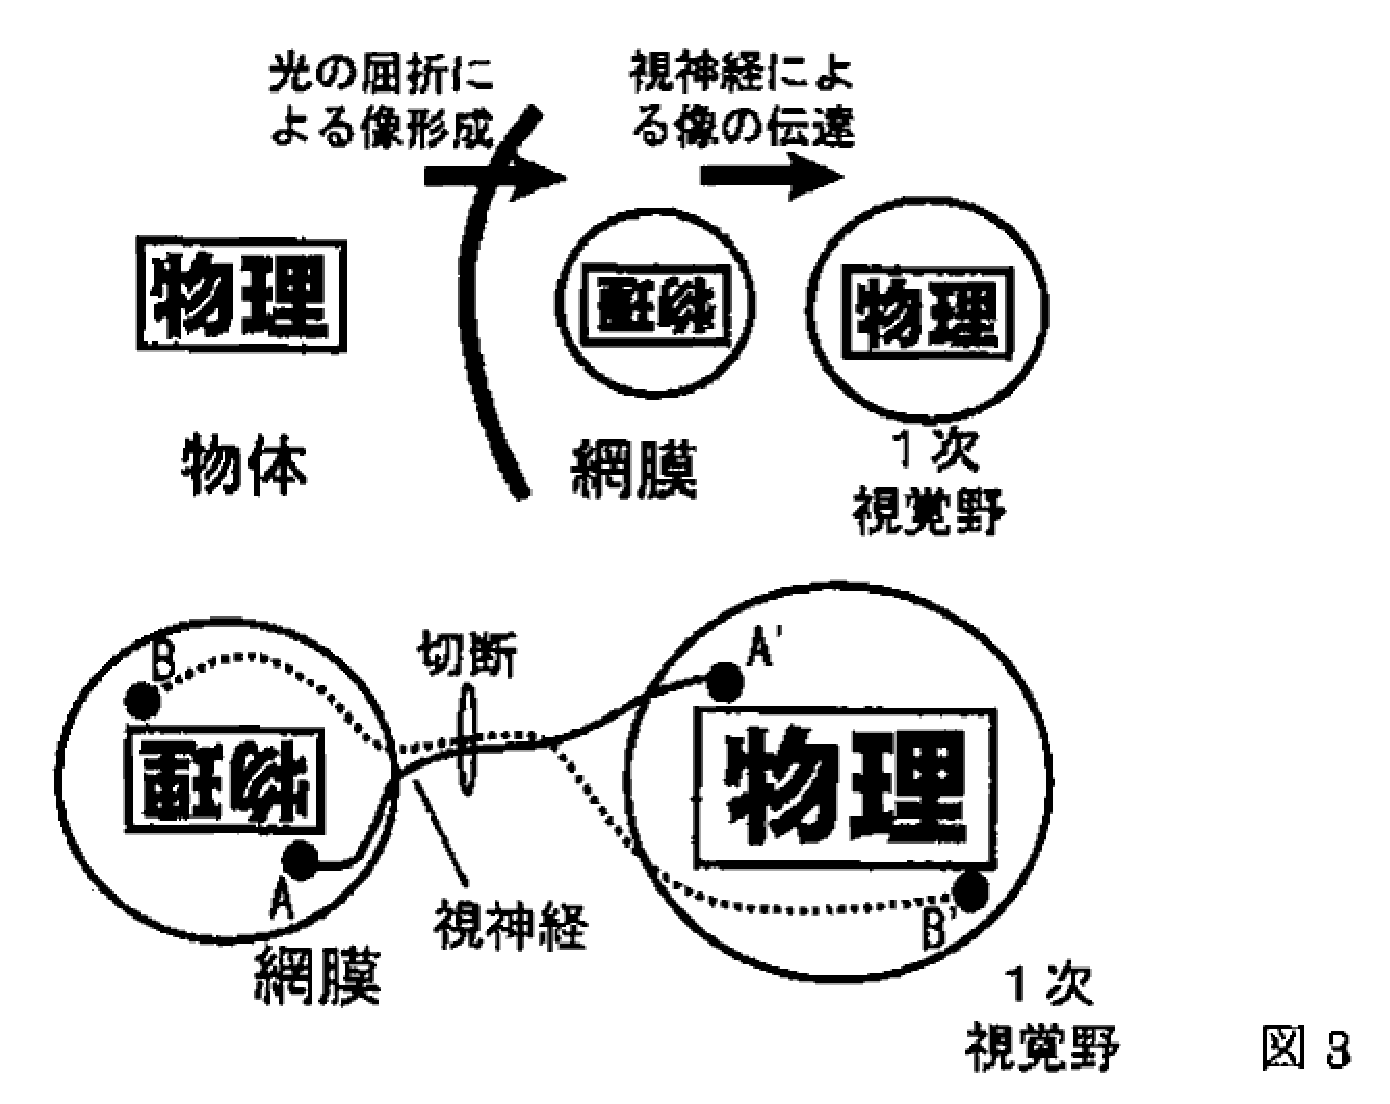
\includegraphics[width=100mm]{2003phy8-3.eps}
\end{center}
\end{figure}

\end{enumerate}
\end{question}

\begin{answer}{問題8}{菅原・永村}
\begin{enumerate}
\item $\alpha$、$\beta$、$\gamma \ll 1$より、$\alpha \simeq \tan \alpha = h/p$、以下$\beta$、$\gamma$も同様に考えて
\begin{eqnarray}
\alpha = \frac{h}{p} \qquad \beta = \frac{h}{q} \qquad \gamma = \frac{h}{r}
\end{eqnarray}
\item 異なる媒質の境界における入射角、屈折角、媒質の屈折率の関係式は、$\theta_1$、$\theta_2$、$n_1$、$n_2$を用いて
\begin{eqnarray}
n_1 \sin \theta_1 = n_2 \sin \theta_2
\end{eqnarray}
と書ける。$\theta_1$、$\theta_2 \ll 1$より、$\sin \theta_1 \simeq \theta_1$、$\sin \theta_2 \simeq \theta_2$から、
\begin{eqnarray}
\frac{\theta_1}{\theta_2} = \frac{n_2}{n_1}
\end{eqnarray}
\item $\triangle$ABCに注目すると、$\theta_1 = \alpha + \gamma$、$\triangle$IBCに注目すると、$\theta_2 = \gamma - \beta$ \\
設問2の結果$n_1 \theta_1 = n_2 \theta_2$から$n_1 (\alpha + \beta) = n_2 (\gamma - \beta)$ \\
これに設問1の値を代入し、両辺に出てくる$h$を消去して、
\begin{eqnarray}
n_1 (\frac{1}{p} + \frac{1}{r}) = n_2 (\frac{1}{r} - \frac{1}{q})
\end{eqnarray}
\item 設問3で得られた式を変形して、
\begin{eqnarray}
r = \frac{(n_2 - n_1)pq}{n_1 q + n_2 p}
\end{eqnarray}
像の拡大率$m$は
\begin{eqnarray}
m = \frac{y'}{y} = \frac{q-r}{p+r} = \frac{q - \frac{(n_2 - n_1)pq}{n_1 q + n_2 p}}{p + \frac{(n_2 - n_1)pq}{n_1 q + n_2 p}} = \frac{(n_1 q + n_2 p)q - (n_2 - n_1)pq}{(n_1 q + n_2 p)p + (n_2 - n_1)pq} = \frac{n_1 q}{n_2 p}
\end{eqnarray}
ゆえに、
\begin{eqnarray}
m = \frac{n_1 q}{n_2 p}
\end{eqnarray}
\item 設問3で得られた式を変形して、
\begin{eqnarray}
q = \frac{\frac{n_2}{n_1}}{(\frac{n_2}{n_1}-1)\frac{1}{r}-\frac{1}{p}}
\end{eqnarray}
問題に与えられているように、
$n_2/n_1 = 1.34$、$1/r = 1/0.80 = 1.25 \> $(1/cm)なので、
\begin{eqnarray}
q = \frac{1.34}{0.34 \times 1.25 -\frac{1}{p}}
\end{eqnarray}
$p = 25 \> $(cm)のとき、$1/p = 0.04 \> $(1/cm)
\begin{eqnarray}
q_{\mbox{{\tiny opt}}} = \frac{1.34}{0.34 \times 1.25 - 0.04} = 3.48 \cdots \simeq 3.5
\end{eqnarray}
$p = \infty $のとき、$1/p = 0$
\begin{eqnarray}
q_{\mbox{{\tiny inf}}} = \frac{1.34}{0.34 \times 1.25} = 3.15 \cdots \simeq 3.2
\end{eqnarray}
したがって、
$p = 25 \> $(cm)のとき$q_{\mbox{{\tiny opt}}} = 3.5 \> $(cm)、
$p = \infty \> $のとき$q_{\mbox{{\tiny int}}} = 3.2 \> $(cm)
\item 設問5で求めた$q$の値は、いずれも角膜と網膜との間の実際の距離2.5cmよりも大きいため、網膜上に像を結ぶようにするためには、像を近くに結ぶためのレンズとしての働きを持つ器官が必要であり、これが水晶体である。設問5の結果からわかるように、物体との距離は見る対象によって変化し、それに応じて空気と角膜の間の屈折だけを考えた時に像を結ぶ位置は変化するので、像の位置を網膜上に持っていくためにレンズとしての水晶体は焦点距離を変化させる必要がある。これは水晶体を周りで支えるチン小体と毛様筋の弛緩・収縮と水晶体自身の弾性により、水晶体の厚みを変化させることで対応している。物体との距離が近いほど、より近くに像を結ぶために、水晶体は厚くなり、レンズとしての焦点距離は短くなる。
\item 孵化後間もなく目を手術して上下さかさまに移植し直し、視覚情報を学習できないようにしばらく暗室で生育させた視神経再生後のカエルを用いる。簡単なところでは、まずこのカエルを明るい場所に移してエサを与え、エサが取れるかどうか観察してみればよい。エサがまともに取れなかったら、正しい配線パターンは学習により獲得されるものどと結論づけられる。これだけだと、エサが取れた場合には他の感覚に依存している可能性がある。人間の脳における学習のように、カエルの視神経の配線パターンが後天的に獲得されるなら、暗い場所で生育されていて視覚情報の学習できなかった時期に確立された配線パターンから、明るい場所で生育されている過程において正しく配線がつなぎ変わることが予想される。したがって、ある図形を見せたときに脳内において電気信号が伝わって来て刺激を受信する位置を何らかの方法\footnote{視野地図は実際に2DG(2-デオキシグルコース)法を用いて可視化することができる。細胞は、放射性ラベルした2DGをグルコースと区別することなく取り込むが、代謝することはできず、オートラジオグラフィーにより、貯留した2DGを可視化することができる。高い活動を示し、エネルギー源として多くのグルコースを必要とする細胞が高くラベルされる。}でマーキングし、暗室から出した直後と、しばらく明るい場所で生育させた後で、脳内で信号が観測される部位の位置パターンに変化があるか調べればよい。変化があれば、配線パターンは学習によって獲得されるものであり、変化がなければ、遺伝的にプログラムされたものである。
\item 各視神経と一次視覚野の特定の位置を対応づける分子があったとしても、一対一対応であると考えることは不可能である。考えられる機構として、\\
1.細胞間接着力に勾配がある。 \\
2.少数の物質が、場所によって濃度勾配を形成しており、これが視神経の結合部位に影響を与えている。 \\
前者の場合、場所により接着力が異なるとなると、マッピングがうまく維持できない可能性がある\footnote{例えばプラモデルを作るときに、はじめから接着剤をべたべた塗ってしまうとうまく作れないであろう。あらかじめパーツをはめてくっつくべきところを確認してから接着しないといけない。これは生体内の細胞接着でも同じことである。}ので、後者のように考えるのが自然である\footnote{この考え方自体は実際に昔からあったらしいが、実験的に解明され始めたのは1995年とごく最近のことである。この実験結果は、『網膜の神経細胞は、鼻から耳方向に行くにつれてEphA3というレセプター分子の密度が高くなり、中脳視蓋(一次視覚野は大脳にある部位だが、その中継部位)ではこのレセプターに結合するephrin-A2というリガンド分子の密度が前から後ろに行くに従って高くなっており、レセプター密度の低い視神経はリガンド密度の高い視蓋細胞表面と結合いていた』というものである。レセプターにリガンドが結合することで細胞にシグナルを伝達するのだが、フリーのレセプターとリガンドが十分量存在して、レセプター、リガンドの結合、解離が平衡反応だとすると、単純な化学反応論に従うとしてよい。すると、レセプター密度$R$、リガンド密度$L$として、シグナルの強さは$R \cdot L$と考えてよい。網膜の各場所から出た視細胞は、共通のシグナル強度の標準値$S$を持つとすると、視神経の軸索先端の成長円錐は今受けているシグナル強度$R \cdot L$と、標準値$S$との差が小さくなるようにサーボしながら動く、という仮定を考えることができる。これをサーボ機構モデルといい、視神経のマッピングにおける最近の有力なモデルである。勿論生体内ではさらに正確なマッピングのための様々な機構が働いていることが予測される。ただし、院試ではここまでの知識は要求されないと思うが…。}。

\bigskip

記述部分の解答には確固たる自信はありません。もし間違っていたらごめんさい…m(\_ \_)m 適当に自分で訂正を入れて下さい。

\end{enumerate}
\end{answer}

\end{document}
